%%%%%%%%%%%%%%%%%%%%%%%%%%%%%%%%%%%%%%%%%
% Journal Article
% LaTeX Template
% Version 1.3 (9/9/13)
%
% This template has been downloaded from:
% http://www.LaTeXTemplates.com
%
% Original author:
% Frits Wenneker (http://www.howtotex.com)
%
% License:
% CC BY-NC-SA 3.0 (http://creativecommons.org/licenses/by-nc-sa/3.0/)
%
%%%%%%%%%%%%%%%%%%%%%%%%%%%%%%%%%%%%%%%%%
%----------------------------------------------------------------------------------------
%       PACKAGES AND OTHER DOCUMENT CONFIGURATIONS
%----------------------------------------------------------------------------------------
\documentclass[paper=letter, fontsize=10pt]{article}
\usepackage[english]{babel} % English language/hyphenation
\usepackage{amsmath,amsfonts,amsthm} % Math packages
\usepackage[utf8]{inputenc}
\usepackage{blindtext, subcaption, caption, graphicx, float, hyperref, tikz, pgfplots}
% float: Required for tables and figures in the multi-column environment - they need to be placed in specific locations with the [H] (e.g. \begin{table}[H])
% Hyperref: For hyperlinks in the PDF
\usepackage[sc]{mathpazo} % Use the Palatino font
\usepackage[T1]{fontenc} % Use 8-bit encoding that has 256 glyphs
\linespread{1.05} % Line spacing - Palatino needs more space between lines
\usepackage{microtype} % Slightly tweak font spacing for aesthetics
\usepackage[hmarginratio=1:1,top=32mm,columnsep=20pt]{geometry} % Document margins
\usepackage{multicol} % Used for the two-column layout of the document
%\usepackage[hang, small,labelfont=bf,up,textfont=it,up]{caption} % Custom captions under/above floats in tables or figures
\usepackage{booktabs} % Horizontal rules in tables
\usepackage{lettrine} % The lettrine is the first enlarged letter at the beginning of the text
\usepackage{paralist} % Used for the compactitem environment which makes bullet points with less space between them
\usepackage{abstract} % Allows abstract customization
\renewcommand{\abstractnamefont}{\normalfont\bfseries} % Set the "Abstract" text to bold
\renewcommand{\abstracttextfont}{\normalfont\small\itshape} % Set the abstract itself to small italic text
\usepackage{titlesec} % Allows customization of titles

\renewcommand\thesection{\Roman{section}} % Roman numerals for the sections
\renewcommand\thesubsection{\Roman{subsection}} % Roman numerals for subsections

\titleformat{\section}[block]{\large\scshape\centering}{\thesection.}{1em}{} % Change the look of the section titles
\titleformat{\subsection}[block]{\large}{\thesubsection.}{1em}{} % Change the look of the section titles
\newcommand{\horrule}[1]{\rule{\linewidth}{#1}} % Create horizontal rule command with 1 argument of height
\usepackage{fancyhdr} % Headers and footers
\pagestyle{fancy} % All pages have headers and footers
\fancyhead{} % Blank out the default header
\fancyfoot{} % Blank out the default footer

\fancyhead[C]{University of Southern Denmark $\bullet$ RM-UAST $\bullet$ Spring 2017 $\bullet$ Group 5 } % Custom header text

\fancyfoot[RO,LE]{\thepage} % Custom footer text
%----------------------------------------------------------------------------------------
%       TITLE SECTION
%----------------------------------------------------------------------------------------
\title{\vspace{-15mm}\fontsize{24pt}{10pt}\selectfont\textbf{Module Eight }} % Article title
\author{
\large
{\textsc{}}\\[2mm]
{\textsc{Henrik Frank, hefra13@student.sdu.dk }}\\[2mm]
{\textsc{Christian Arentsen, chare13@student.sdu.dk }}\\[2mm]
{\textsc{Vasileios Karvouniaris, vakar15@student.sdu.dk }}\\[2mm]
{\textsc{Asbjørn Schou Müller, asmul10@student.sdu.dk }}
%\thanks{A thank you or further information}\\ % Your name
%\normalsize \href{mailto:marco.torres.810@gmail.com}{marco.torres.810@gmail.com}\\[2mm] % Your email address
}
\date{}

%----------------------------------------------------------------------------------------
\begin{document}
\maketitle % Insert title
\thispagestyle{fancy} % All pages have headers and footers

\section{Exercises}

\subsection{Radio link budget}
The objective of this exercise is to learn about radio link budgets and how they may be applied when designing radio communication systems for drones.

\subsubsection{Unit conversion mW and dbm}

What is the unit conversion between power expressed in mW and dBm? What is the value in dBm for 100mW, 500mW and 1W?

\paragraph{Result} 1mW is relative to 1dBm. Rule of thumb; double the power = 3dBm increase, half the power = 3dBm decrease

\begin{equation*}
dB = 10*log_10 \frac{P_1}{P_2}
\end{equation*}

\begin{tabular}{| l | l | }
  100 mW & 20 dBm \\
  500 mW & 27 dBm \\
  1W & 30 dBm
\end{tabular}

\subsubsection{Free-space basic transmission loss}
\label{sec:freesp}
The \textit{free-space basic transmission loss} (attenuation) $L_{bf}$ expressed in $dB$ in equation \ref{eq:freespaceloss} where $P_r$ is the power received by an isotropic antenna, $P_t$ is the power transmitted by an isotropic antenna, $f$ is the frequency in MHz, $d$ is the distance in meter between transmitter and receiver \footnote{RECOMMENDATION ITU-R P.525-2}. 

\begin{eqnarray}
\frac{P_t}{P_r} &=& \left(\frac{4 \pi f d}{300}\right)^2 \\
L_{bf} &=& 10 \, log_{10}\left(\frac{4 \pi f d}{300}\right)^2 = 20 \, log_{10}\left(\frac{4 \pi f d}{300}\right) \\
&\approx& -27.55 + 20 \, log_{10} (f) + 20 \, log_{10}\left(d\right)
\label{eq:freespaceloss}
\end{eqnarray}

Please explain in words what is free-space basic transmission loss and what physical properties contributes to this?


Free-space basic transmission loss (FSPL) is the power loss that would occur on a line-of-sight path through space, without being affected by reflection or refraction. Usually expressed in dB, although the IEEE standard does not say that.\cite{wiki} The main properties of FSPL are the transmission distance and the frequency of the signal. 


\subsubsection{Radio link budget}
A radio link budget contains the following factors listed below expressed in decibels. Optionally the calculation may include Bit Error Rate (BER) for digital links.

\begin{enumerate}
	\item The transmitted power level
	\item Signal loss as it travels to the receiver (free-space)
	\item Frequency band background noise level (what is the minimum SNR that will allow the receiver to extract a usable signal).
	\item How the transmitting and receiving antenna systems shape the signal
	\item Receiver sensitivity
\end{enumerate}


Please create (and document) a radio link budget for a a 2.4 GHz C2 link, a 433 MHz telemetry link and a 5.8 GHz video downlink respectively. This is not a trivial task, and you may want to search the web for examples of radio link budgets. The course materials for this module contains a few references as well.

\paragraph{Results} Please refer to the spreadsheet included in the hand\-in folder, thank you. 

\subsection{Near field absorption and Fresnel zones}
The objective of this exercise is to learn about near field absorption and Fresnel zones and how they relate to drone technology.


\subsubsection{Near field absorptions}
Please explain what is \textit{near field absorption} and to the extent possible based on information available on the web please quantify the signal attenuation.



\subsubsection{Fresnel zones}
Please explain in details using a sketch or an image from the web what is a Fresnel zone (equation \ref{eq:fresnel}) and how does it relate to drone C2 and telemetry links?


\begin{equation}
F_n = \sqrt{\frac{n\, \lambda \, (d_1\, d_2)}{d_1 + d_2}}
\label{eq:fresnel}
\end{equation}

Fresnel zones are a series of prolate ellipsoidal regions of space between and around a transmitting antenna and a receiving antenna system.\cite{wikipedia_fresnel}. The equation above\ref{eq:fresnel} is used for calculating the Fresnel zone radius at any point P in between the transmitting and the receiving antennas. \textit{$F_n$} is the radius of the zone, \textit{$d_1$} is the distance of P from one end-point, \textit{$d_2$} and $\lambda$ is the wavelength of the transmitted signal.

\begin{figure}[h!]
\centering
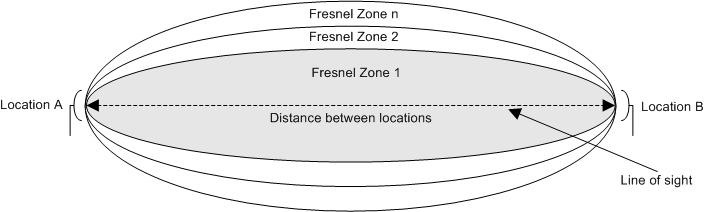
\includegraphics[scale=1.5]{Figures/Fresnel_zones}
\caption{Graph of Fresnel zones}
\label{fig:fresnel_zones}
\end{figure}


\subsubsection{Plotting Fresnel zones}
Using Python please plot the Fresnel zones for a 2.4 GHz C2 link, a 433 MHz telemetry link and a 5.8 GHz video downlink respectively. 

\subsubsection{Fresnel zone loss}
Assuming that the greatest Fresnel zone losses occur when a diffracting object blocks about 40\% of the 1st Fresnel zone. Please calculate and discuss what this means to a drone at a height of 50m with respect to the ground at 400m distance from an operator sitting on the ground holding the TX at an approx height of 0.5m.

Please consider another situation where a standing drone operator controls a drone at 200m distance. The drone is visible just above the ride line of the metal roof of a building at a distance of 30 meter. How much visual clearance must there be between the direct line of sight and the ridge line to ensure that the first Fresnel zone is clear for a 2.4 GHz C2 link, a 433 MHz telemetry link and a 5.8 GHz video downlink respectively?


\subsection{Path loss model based on terrain contours}

Use the \href{http://www.sws.bom.gov.au/Category/HF\%20Systems/Online\%20Tools/Prediction\%20Tools/VUHF/VUHF.php}{VHF/UHF Area Prediction Tool} to model path loss influenced by the terrain contours. Is the result comparable to the free space loss estimated in exercuse \ref{sec:freesp} if you select HCA Airport as location (N55.47036, E010.32967)? What if you select Svanninge Bakker (N55.12518, E010.25419)?

%\pagebreak

\bibliographystyle{plain}
%https://en.wikipedia.org/wiki/Line-of-sight_propagation
\bibliography{bibfile}
%----------------------------------------------------------------------------------------
%\end{multicols}
\end{document}
